\documentclass[11pt,a4paper]{article}
\PassOptionsToPackage{hyphens}{url}

% =====================================================================
%   PAKETLER (Önce paketler yüklenmelidir)
% =====================================================================
\usepackage[utf8]{inputenc}
\usepackage[T1]{fontenc}
\usepackage[a4paper,left=2.7cm,right=2.7cm,top=2.8cm,bottom=2.8cm,headsep=12pt,headheight=14pt]{geometry}
\IfFileExists{lmodern.sty}{\usepackage{lmodern}}{}
\IfFileExists{lmodern.sty}{\usepackage{microtype}}{\usepackage[expansion=false]{microtype}}

\usepackage{etoolbox}
\usepackage{graphicx}
\usepackage{xcolor}
\usepackage{titlesec}
\usepackage{titling}
\usepackage{fancyhdr}
\usepackage{enumitem}
\usepackage{booktabs}
\usepackage{array}
\usepackage{caption}
\usepackage{subcaption}
\usepackage{amsmath,amssymb}
\usepackage{listings}
\usepackage{tcolorbox}
\tcbuselibrary{skins,breakable}
\usepackage[hidelinks]{hyperref}
\usepackage[capitalise]{cleveref}
\usepackage{csquotes}
\usepackage{setspace}
\usepackage{tabularx}
\usepackage{multirow}
\usepackage{float}
\usepackage{tikz}
\usetikzlibrary{positioning,arrows.meta}
\usepackage[numbers,sort&compress]{natbib}
\setlength{\emergencystretch}{2em}

\usepackage[shorthands=off,turkish,english]{babel}

% =====================================================================
%   KONTROL BAYRAĞI / CONTROL FLAG
% =====================================================================
%   DİL VE DERS BAYRAĞI:
%     1 = Türkçe kapak / üst bilgi / başlıklar ve BLM3010 -- Bilgisayar Projesi
%     0 = İngilizce kapak / üst bilgi / başlıklar ve BLM9000 -- Bitirme Çalışması
%    Aşağıdaki DILBAYRAGI{1} kısmını dersinize göre 0 ya da 1 olarak derse göre seçiniz
% -------------------------------------------------------------
\def\DILBAYRAGI{1}

\newtoggle{TURKCE}
\newtoggle{BLMUC}

\ifnum\DILBAYRAGI=1
  \toggletrue{TURKCE}
  \togglefalse{BLMUC}
  \selectlanguage{turkish}
\else
  \togglefalse{TURKCE}
  \togglefalse{BLMUC}
  \selectlanguage{english}
\fi

% --- Dil bayrağına göre İçindekiler / Şekil / Tablo başlıkları ---
\iftoggle{TURKCE}{
  \renewcommand{\contentsname}{İçindekiler}
  \renewcommand{\listfigurename}{Şekiller}
  \renewcommand{\listtablename}{Tablolar}
  \renewcommand{\figurename}{Şekil}
  \renewcommand{\tablename}{Tablo}
}{
  \renewcommand{\contentsname}{Contents}
  \renewcommand{\listfigurename}{List of Figures}
  \renewcommand{\listtablename}{List of Tables}
  \renewcommand{\figurename}{Figure}
  \renewcommand{\tablename}{Table}
}

% =====================================================================
%   RENK PALETİ
% =====================================================================
\definecolor{anacolor}{RGB}{0,0,0}
\definecolor{vurgucolor}{RGB}{0,0,0}
\definecolor{acikgri}{RGB}{245,245,245}
\definecolor{kodgri}{RGB}{250,250,250}
\definecolor{cizgi}{RGB}{0,0,0}

% =====================================================================
%   BAŞLIK BİÇİMLERİ
% =====================================================================
\titleformat{\section}
  {\normalfont\Large\bfseries\color{anacolor}}
  {\thesection}{0.6em}{}
  [\vspace{-2pt}{\color{cizgi}\titlerule[1.1pt]}]

\titleformat{\subsection}
  {\normalfont\large\bfseries\color{anacolor!85!black}}
  {\thesubsection}{0.6em}{}

\titleformat{\subsubsection}
  {\normalfont\normalsize\bfseries\color{vurgucolor}}
  {\thesubsubsection}{0.6em}{}

\titlespacing*{\section}{0pt}{22pt}{12pt}
\titlespacing*{\subsection}{0pt}{14pt}{8pt}
\titlespacing*{\subsubsection}{0pt}{10pt}{6pt}

% =====================================================================
%   ÜST / ALT BİLGİ (HEADER / FOOTER)
% =====================================================================
\pagestyle{fancy}
\fancyhf{}
\renewcommand{\headrulewidth}{0.6pt}
\renewcommand{\footrulewidth}{0.3pt}
\fancyhead[L]{\small\color{gray}\projebasligikisa}
\fancyhead[R]{\small\color{gray}\nouppercase{\leftmark}}
\fancyfoot[C]{\small\color{gray}\thepage}

\fancypagestyle{ilksayfa}{
  \fancyhf{}
  \fancyfoot[C]{\small\color{gray}\thepage}
  \renewcommand{\headrulewidth}{0pt}
  \renewcommand{\footrulewidth}{0.3pt}
}

% =====================================================================
%   KOD BLOKLARI (listings)
% =====================================================================
\lstdefinestyle{kodstil}{
  backgroundcolor=\color{kodgri},
  basicstyle=\ttfamily\small,
  keywordstyle=\color{anacolor}\bfseries,
  commentstyle=\color{gray}\itshape,
  stringstyle=\color{vurgucolor},
  numberstyle=\tiny\color{gray},
  numbers=left,
  numbersep=8pt,
  frame=single,
  rulecolor=\color{cizgi},
  framesep=6pt,
  breaklines=true,
  showstringspaces=false,
  tabsize=2,
  captionpos=b
}
\lstset{style=kodstil}

% =====================================================================
%   BİLGİ KUTUSU
% =====================================================================
\newtcolorbox{bilgikutu}[1][]{
  colback=acikgri, colframe=anacolor,
  boxrule=0.6pt, arc=2pt, left=8pt, right=8pt, top=6pt, bottom=6pt,
  fonttitle=\bfseries\color{white}, colbacktitle=anacolor,
  #1
}

% =====================================================================
%   KAPAK SAYFASI METİNLERİ / COVER PAGE TEXT
% =====================================================================
\newcommand{\txtUniversite}{\iftoggle{TURKCE}{YILDIZ TEKNİK ÜNİVERSİTESİ}{YILDIZ TECHNICAL UNIVERSITY}}
\newcommand{\txtFakulte}{\iftoggle{TURKCE}{ELEKTRİK-ELEKTRONİK FAKÜLTESİ}{Faculty of Electrical and Electronics}}
\newcommand{\txtBolum}{\iftoggle{TURKCE}{Bilgisayar Mühendisliği Bölümü}{Department of Computer Engineering}}

\newcommand{\txtRaporTuru}{%
  \iftoggle{BLMUC}{%
    \iftoggle{TURKCE}{BLM3010 -- Bilgisayar Projesi}{BLM3010 -- Computer Project}%
  }{%
    \iftoggle{TURKCE}{BLM9000 -- Bitirme Çalışması}{BLM9000 -- Graduation Thesis}%
  }%
}

\newcommand{\txtOgrenciNo}{\iftoggle{TURKCE}{Öğrenci No}{Student ID}}
\newcommand{\txtDanismanEt}{\iftoggle{TURKCE}{Danışman}{Advisor}}
\newcommand{\txtAyYil}{\iftoggle{TURKCE}{Kasım 2026}{November 2026}}

% =====================================================================
%   BAŞLIK / YAZAR BİLGİLERİ
% =====================================================================
\newcommand{\projebasligikisa}{\txtRaporTuru}

\title{\vspace{-1.2cm}
  {\color{anacolor}\rule{\linewidth}{1.3pt}}\\[10pt]
  {\Huge\bfseries\color{anacolor} ARTIRILMIŞ GERÇEKLİK DESTEKLİ\\[4pt] MOBİL ROBOT OYUNU}\\[6pt]
  {\color{anacolor}\rule{\linewidth}{1.3pt}}\\[4pt]
  {\normalsize \txtBolum\ -- \txtRaporTuru}
}

\author{
  \large \textbf{İsa Koçan} \\[2pt]
  \small \txtOgrenciNo: 22011056\\[6pt]
  \large \textbf{Bilal Efe Uysal} \\[2pt]
  \small \txtOgrenciNo: 22011031\\[10pt]
  \large \textbf{\txtDanismanEt:} Dr. Öğr. Üyesi Furkan Çakmak \\[14pt]
  \normalsize \txtUniversite \\
  \normalsize \txtFakulte\ -- \txtBolum
}

\date{\normalsize \txtAyYil}

% =====================================================================
%   BELGE BAŞLANGICI
% =====================================================================
\begin{document}

\pagenumbering{gobble}

\begin{titlepage}
\thispagestyle{empty}
\begin{center}
\vspace*{0cm}


\includegraphics[width=3.5cm]{assets/logo.png}\\[0.8cm]

{\large \txtUniversite}\\[2pt]
{\large \txtFakulte}\\[2pt]
{\large \txtBolum}\\[1.2cm]

{\color{anacolor}\rule{0.85\linewidth}{1.4pt}}\\[14pt]
{\LARGE\bfseries\color{anacolor} ARTIRILMIŞ GERÇEKLİK DESTEKLİ\\[4pt] MOBİL ROBOT OYUNU}\\[14pt]
{\color{anacolor}\rule{0.85\linewidth}{1.4pt}}\\[1.1cm]

{\Large \txtRaporTuru}\\[1.2cm]

\begin{tabular}{c}
\large \textbf{Bilal Efe Uysal} \\
\small \txtOgrenciNo: 22011031 \\[6pt]
\large \textbf{İsa Koçan} \\
\small \txtOgrenciNo: 22011056
\end{tabular}\\[1cm]

\begin{tabular}{c}
\large \textbf{\txtDanismanEt} \\
Dr. Öğr. Üyesi Furkan Çakmak
\end{tabular}

\vfill

{\normalsize \txtAyYil}\\[0.4cm]

\end{center}
\end{titlepage}

\pagenumbering{roman}
\setcounter{page}{2}

% ---------------- ÖNSÖZ ----------------
\section*{Önsöz}
\addcontentsline{toc}{section}{Önsöz}
Yapay zekâ, görüntü işleme ve artırılmış gerçeklik gibi alanlar günlük hayatımıza hızla girerken, gerçek dünya ile dijital dünyayı birleştiren sistemler hem bilimsel hem de eğlence açısından büyük ilgi görmektedir. Bu çalışma, fiziksel bir robotu telefondan sürerken robotun gördüğü ortamı sanal nesnelerle zenginleştiren bir oyun fikrinden doğmuştur. Amacımız, bir sistemi donanımdan yazılıma, görüntü aktarımından robotun konumunu bulmaya kadar baştan sona kurmak ve bunu herkesin kolayca oynayabileceği bir deneyime dönüştürmekti. Çalışma yapay zekâ ve görüntü işleme, gömülü sistemler, haberleşme ve oyun geliştirme gibi birbirinden farklı alanları tek bir sistemde bir araya getirmektedir.

Çalışma boyunca birçok alanda yeni şeyler öğrendik. Robotun mekanik ve elektronik yapısıyla uğraşırken donanımın gerçek dünyadaki sınırlarıyla karşılaştık. Düşük gecikmeli görüntü aktarımı, kablosuz haberleşme ve güvenli sürüş gibi konularda deneyim kazandık. Yapay zekâ ile görüntü işleme, konum belirleme ve oyun geliştirme üzerine okuduğumuz çalışmalar bize yeni bakış açıları kazandırdı. Bunların yanında bir ekip olarak iş bölümü yapmayı, farklı fikirleri bir araya getirmeyi ve ortak bir hedefe doğru ilerlemeyi öğrendik.

Bu süreçte bize yol gösteren danışman hocamız Dr. Öğr. Üyesi Furkan Çakmak'a içtenlikle teşekkür ederiz. Robotun fiziksel olarak oluşturulmasında hocamızın katkısı belirleyici olmuştur. Tüm parçaları temin etmiş, montaj sürecinde bilgi ve tecrübesiyle bize yol göstermiş ve karşılaştığımız sorunlarda önerileriyle destek olmuştur. Bilgi ve deneyimini bizimle paylaşmaktan çekinmediği ve çalışmamıza verdiği destek için ona büyük bir minnet duyuyoruz.

Eğitim hayatımız boyunca ve bu çalışma sırasında bizi her zaman destekleyen, bize güvenen ve sabır gösteren ailelerimize en içten teşekkürlerimizi sunarız. Denemelerimiz sırasında bize zaman ayıran, fikirleriyle ve desteğiyle yanımızda olan arkadaşlarımıza da ayrıca teşekkür ederiz. Onların desteği olmadan bu çalışmayı bu noktaya getirmemiz mümkün olmazdı.

Bu çalışmayı hazırlarken, aklı ve bilimi yol gösterici kabul eden Cumhuriyetimizin kurucusu Gazi Mustafa Kemal Atatürk'ü saygı, minnet ve özlemle anıyoruz. Ülkemizi çağdaş uygarlık düzeyinin üzerine çıkarma hedefiyle eğitime ve bilime verdiği değer, bizim gibi genç mühendis adaylarına da yol göstermektedir. Bugün üniversitede öğrenim görebiliyor ve bilimsel çalışma yapabiliyorsak, bunu onun kurduğu Cumhuriyet'e ve bu yolda emek veren herkese borçluyuz. Onun gösterdiği hedefler doğrultusunda çalışmaya, üretmeye ve ülkemize faydalı olmaya devam etmeyi görev biliriz.

\vspace{1.2cm}
\noindent\hfill Bilal Efe Uysal, İsa Koçan\\
\hspace*{\fill}Kasım 2026

\newpage

% ---------------- ÖZET VE ABSTRACT ----------------
\section*{Özet}
\addcontentsline{toc}{section}{Özet}
Bu bölüm daha sonra doldurulacaktır.

\vspace{1cm}

\section*{Abstract}
\addcontentsline{toc}{section}{Abstract}
This section will be completed later.

\newpage
% ---------------- İÇİNDEKİLER ----------------
\selectlanguage{turkish}
\tableofcontents
\newpage
\listoffigures
\listoftables
\newpage

\pagenumbering{arabic}
\setcounter{page}{1}

% =====================================================================
%   BÖLÜM-1: GİRİŞ
% =====================================================================
\section{Giriş / Introduction}
\label{sec:giris}
Bu bölümde projenin amacı ve kapsamı anlatılmış, ardından ilgili çalışmalar incelenmiştir.

\subsection{Amaç ve Kapsam / Aim and Scope}
\label{subsec:amac_kapsam}
Artırılmış gerçeklik (augmented reality, AR) oyunlarında sanal içerik gerçek ortamın üzerine yerleştirilir, ancak gerçek ortamda hareket eden tek şey genellikle oyuncunun kendisidir. Oyuna fiziksel bir robot katılırsa deneyim zenginleşir, fakat sanal nesneleri doğru yere koymak için robotun ortamdaki yerini bilmek gerekir. Düşük maliyetli robotlarda ise konum sensörleri çoğunlukla bulunmaz.

Bu projede, telefondan sürülen 360° kameralı bir robotla ev içinde oynanan bir AR oyunu geliştiriyoruz. Çıkış noktamız, uzaktan kumandalı araçların kamera görüntüsüne sanal öğeler ekleyen Mario Kart Live \cite{mariokartlive2020} oldu. Biz oyunu yarış yerine Pokémon GO \cite{paavilainen2017pokemon} gibi keşfe dayalı kurguluyoruz. Pokémon GO sanal nesneleri küresel konumlama sistemi (global positioning system, GPS) ile gerçek konumlara bağlar. Ev içinde GPS olmadığı için bizde bunun karşılığı odanın haritası ve robotun bu haritadaki konumudur. Robotta bunun için ayrı bir sensör kullanmıyor, konumu yalnızca 360° kamera görüntüsünden bulmayı hedefliyoruz. Bunun için yapay zekâ ve görüntü işleme yöntemlerinden yararlanacağız. Oda haritası bir kez, iPhone'un ışık algılama ve mesafe ölçme (light detection and ranging, LiDAR) sensörüyle ya da LiDAR'sız telefonlarda çift kamerayla çıkarılıp saklanır. Oyun sırasında robotun 360° görüntüsü bu harita içinde eşleştirilerek robotun yeri bulunur.

Projenin hedefleri şunlardır:
\begin{enumerate}[label=H\arabic*.]
  \item Telefondan kablosuz sürülebilen, düşük gecikmeli 360° görüntü aktaran ve bağlantı koptuğunda duran bir robot yapmak.
  \item Odanın haritasını LiDAR ya da çift kamerayla çıkarıp saklamak.
  \item Robotun konumunu 360° görüntüyü bu haritayla eşleştirerek takip etmek.
  \item Konuma bağlı, oynanabilir bir AR oyunu geliştirmek.
\end{enumerate}
Kapsamımız ev gibi kapalı alanlar ve tek oyunculu kullanımdır. Uygulama Unity ile geliştiriliyor ve Android ile iOS'ta çalışacaktır.

\subsection{Literatür Analizi / Literature Review}
\label{subsec:literatur}
İlgili çalışmalar dört başlıkta incelenmiş ve projenin bunlara göre yeri belirtilmiştir.

\paragraph{AR ve robotlu oyunlar.}
Azuma \cite{azuma1997survey}, AR'ı gerçek ve sanal içeriği birleştiren, gerçek zamanlı etkileşimli ve sanal nesneleri gerçek dünyayla hizalayan sistemler olarak tanımlamış, hizalama hatalarını temel sorun olarak göstermiştir. Pokémon GO üzerine yapılan bir çalışma, oyuncuların gerçek dünyayı keşfetmeyi oyunun iyi yanlarından biri olarak gördüğünü göstermiştir \cite{paavilainen2017pokemon}. Pratticò ve Lamberti \cite{prattico2021mixed}, robotu dijital öğelerle birleştiren karma gerçeklik oyunlarının tüketici robotlarının sınırlı oyun seçeneklerini aşabileceğini savunmuştur. Ticari örnek Mario Kart Live'da \cite{mariokartlive2020} oyun alanı odaya konan fiziksel kapı işaretleriyle tanımlanır. Bu ürün bir basın bülteniyle tanıtıldığı için akademik kaynak değildir.

\paragraph{Telefonla oda taraması.}
Luetzenburg ve arkadaşları \cite{luetzenburg2021iphone}, iPhone 12 Pro ve iPad Pro LiDAR sensörlerinin küçük nesnelerde yaklaşık $\pm$1~cm, 130~m uzunluğa kadar büyük alanlarda yaklaşık $\pm$10~cm doğrulukla model üretebildiğini göstermiştir. Apple'ın ARKit kütüphanesi LiDAR'lı cihazlarda ortamı çokgen ağ olarak çıkarır \cite{apple2026arkit}. LiDAR'sız telefonlarda ana ve tele kamerayı birleştiren öğrenme tabanlı derinlik tahmini kullanılabilir \cite{zhang2020dunet}.

\paragraph{Harita içinde kamera ile konum belirleme.}
PICCOLO, tek bir 360° panoramanın renkli bir nokta bulutu içindeki yerini eğitim gerektirmeden bulur \cite{kim2021piccolo}. CPO ise harita çıkarıldıktan sonra sahne değişse bile çalışır \cite{kim2022cpo}, bu da eşyaların sık yer değiştirdiği evler için önemlidir. Konum tahminlerini zamanda takip etmek için Monte Carlo konum belirleme kullanılabilir \cite{dellaert1999mcl}. Yere bakan tek kamerayla yaklaşık 17~m yolda \%0,21 konum hatası elde eden bir görsel odometri çalışması da yalnızca kameradan konum bulmanın mümkün olduğunu gösterir \cite{patruno2020visual}.

\paragraph{360° kameralı uzaktan sürüş.}
Düşük gecikmeli video akışını inceleyen güncel bir derleme, uzaktan sürüşü düşük gecikme gerektiren uygulamalar arasında sayar \cite{tang2026lowlatency}. Telepresence robotunda 360° kamera daha güçlü bir içindelik hissi vermiş, ancak çevre farkındalığı eksik kalmıştır \cite{heshmat2018geocaching}. Bu bulgular, robotun 360° görüntüsünü düşük gecikmeyle telefona aktarmanın oyun deneyimi için kritik olduğunu gösteriyor.

\paragraph{Projenin literatürdeki konumu.}
İncelenen çalışmalar Tablo~\ref{tab:literatur_karsilastirma}'de özetlenmiştir. Konum tabanlı AR oyunları oyuncunun kendi hareketine, robotlu oyunlar dış işaretlere dayanır. Panorama ile harita içinde konum bulan yöntemler ise oyun bağlamında ve düşük maliyetli bir robot üzerinde denenmemiştir. Projemiz oda haritasını oyuncunun telefonuyla çıkarmayı, robotun konumunu ek sensör olmadan yalnızca 360° kamerayla bulmayı ve bunu bir oyunda kullanmayı birleştirir.

\begin{table}[H]
\centering
\caption{İncelenen çalışmaların karşılaştırılması}
\label{tab:literatur_karsilastirma}
\small
\begin{tabularx}{\linewidth}{>{\raggedright\arraybackslash}X c c c >{\raggedright\arraybackslash}X c}
\toprule
\textbf{Çalışma} & \textbf{Robot} & \textbf{360° kamera} & \textbf{AR} & \textbf{Gerçek mekâna bağlama} & \textbf{Oyun} \\
\midrule
Pokémon GO \cite{paavilainen2017pokemon} & -- & -- & \checkmark & Telefonun konumu & \checkmark \\
Mario Kart Live \cite{mariokartlive2020} & \checkmark & -- & \checkmark & Fiziksel kapı işaretleri & \checkmark \\
Heshmat vd. \cite{heshmat2018geocaching} & \checkmark & \checkmark & -- & -- & -- \\
Patruno vd. \cite{patruno2020visual} & \checkmark & -- & -- & Yere bakan kamerayla göreli konum & -- \\
PICCOLO / CPO \cite{kim2021piccolo,kim2022cpo} & -- & \checkmark & -- & Önceden taranmış nokta bulutu & -- \\
Bu proje & \checkmark & \checkmark & \checkmark & Telefonla taranan oda haritası & \checkmark \\
\bottomrule
\end{tabularx}
\end{table}

Raporun geri kalanı şöyle ilerler. Bölüm~\ref{sec:analiz_fizibilite}'de sistemin analizi ve fizibilitesi sunulmuştur. Sistem tasarımı, deneysel sonuçlar ile sonuç ve tartışma bölümleri sonraki aşamalarda sunulacaktır.

% =====================================================================
%   BÖLÜM-2: SİSTEM ANALİZİ VE FİZİBİLİTE
% =====================================================================
\newpage
\section{Sistem Analizi ve Fizibilite / System Analysis and Feasibility}
\label{sec:analiz_fizibilite}
Bu bölümde sistemin bileşenleri, gereksinimleri ve kısıtları çıkarılmış, ardından projenin yazılım, donanım ve zaman açısından yapılabilirliği değerlendirilmiştir.

\subsection{Sistem Analizi / System Analysis}
\label{subsec:sistem_analizi}
Sistem, telefonda çalışan Unity oyun uygulaması ile ondan kablosuz sürülen 360° kameralı robottan oluşur (Şekil~\ref{fig:sistem_bilesenleri}). Robot bilgisayarı (NVIDIA Jetson Nano), evrensel seri veri yolu (universal serial bus, USB) ile bağlı 360° kameranın (Ricoh Theta S) görüntüsünü telefona aktarır ve sürüş komutlarını mikrodenetleyiciye (Arduino Uno) iletir. Mikrodenetleyici doğru akım (direct current, DC) motorlarını, ışık yayan diyotu (light emitting diode, LED) ve buzzer'ı denetler. Oyuncu odayı LiDAR sensörlü bir telefonla bir kez tarar, ardından robotu sürerken uygulama robotun konumunu harita içinde bulur ve sanal nesneleri buna göre yerleştirir (Şekil~\ref{fig:konum_akisi}).

\begin{figure}[H]
\centering
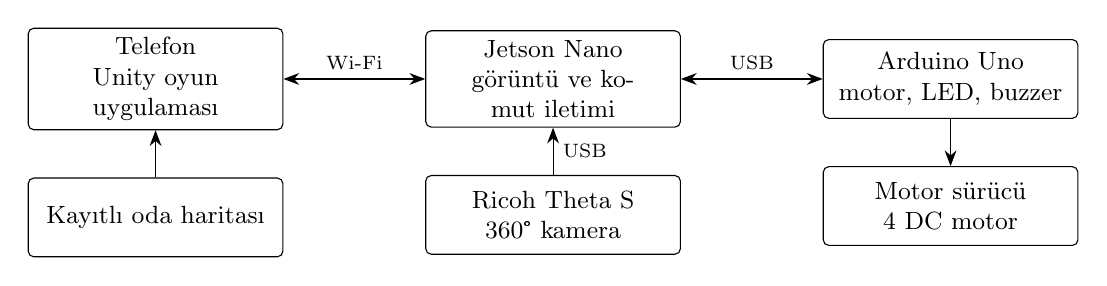
\begin{tikzpicture}[
  box/.style={draw, rounded corners=2pt, minimum height=1cm, text width=3cm, align=center, font=\small},
  >={Stealth[length=2mm]}]
\node[box] (tel) {Telefon\\Unity oyun uygulaması};
\node[box, right=1.8cm of tel] (jet) {Jetson Nano\\görüntü ve komut iletimi};
\node[box, right=1.8cm of jet] (ard) {Arduino Uno\\motor, LED, buzzer};
\node[box, below=0.6cm of tel] (harita) {Kayıtlı oda haritası};
\node[box, below=0.6cm of jet] (cam) {Ricoh Theta S\\360° kamera};
\node[box, below=0.6cm of ard] (mot) {Motor sürücü\\4 DC motor};
\draw[<->] (tel) -- node[above, font=\scriptsize]{Wi-Fi} (jet);
\draw[<->] (jet) -- node[above, font=\scriptsize]{USB} (ard);
\draw[->] (cam) -- node[right, font=\scriptsize]{USB} (jet);
\draw[->] (ard) -- (mot);
\draw[->] (harita) -- (tel);
\end{tikzpicture}
\caption{Sistemin bileşenleri ve aralarındaki bağlantılar}
\label{fig:sistem_bilesenleri}
\end{figure}

\begin{figure}[H]
\centering
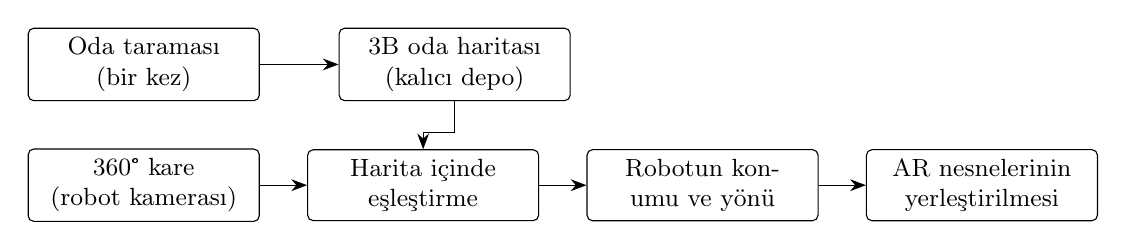
\begin{tikzpicture}[
  box/.style={draw, rounded corners=2pt, minimum height=0.9cm, text width=2.7cm, align=center, font=\small},
  >={Stealth[length=2mm]}]
\node[box] (tara) {Oda taraması\\(bir kez)};
\node[box, right=1cm of tara] (harita) {3B oda haritası\\(kalıcı depo)};
\node[box, below=0.6cm of tara] (kare) {360° kare\\(robot kamerası)};
\node[box, right=0.6cm of kare] (esle) {Harita içinde eşleştirme};
\node[box, right=0.6cm of esle] (konum) {Robotun konumu ve yönü};
\node[box, right=0.6cm of konum] (ar) {AR nesnelerinin yerleştirilmesi};
\draw[->] (tara) -- (harita);
\draw[->] (harita.south) -- ++(0,-0.4) -| (esle.north);
\draw[->] (kare) -- (esle);
\draw[->] (esle) -- (konum);
\draw[->] (konum) -- (ar);
\end{tikzpicture}
\caption{Önerilen konum belirleme akışı}
\label{fig:konum_akisi}
\end{figure}

\paragraph{Gereksinimler ve kısıtlar.}
Fonksiyonel (FG) ve fonksiyonel olmayan (FOG) gereksinimler Tablo~\ref{tab:gereksinimler}'de verilmiştir. Robotta konum sensörü yoktur ve kızaklı sürüşte tekerlekler kaydığı için konum kameradan bulunmalıdır. Oda taraması ile robot kamerası arasındaki yükseklik farkı eşleştirmeyi zorlaştırabilir, LiDAR ise yalnızca bazı cihazlarda bulunur ve menzili sınırlıdır \cite{luetzenburg2021iphone}.

\paragraph{Girdi, çıktı ve ölçütler.}
Girdiler sürüş komutları, derinlik verisi ve 360° görüntü, çıktılar ise oda haritası, robotun konumu, AR görüntüsü ve robota giden komutlardır. Başarım konum hatası (cm), görüntü gecikmesi (ms), bağlantı kopma sayısı ve tam bataryayla oyun süresi (dakika) ile ölçülecek, ayrıca oyun deneyimi, katılımcılara oyun oynatılarak ve kendilerinden 10 üzerinden puan alınarak değerlendirilecektir.

\begin{table}[H]
\centering
\caption{Sistemin gereksinimleri}
\label{tab:gereksinimler}
\small
\begin{tabularx}{\linewidth}{l >{\raggedright\arraybackslash}X}
\toprule
\textbf{Kod} & \textbf{Gereksinim} \\
\midrule
FG-1 & Uygulama robotu ağda kendiliğinden bulup bağlanmalı, oyuncu robotu sürebilmeli ve 360° görüntüde etrafa bakabilmelidir. \\
FG-2 & Oda haritası LiDAR veya çift kamerayla çıkarılmalı ve saklanmalıdır. \\
FG-3 & Robotun konumu harita içinde takip edilmeli, sanal nesneler zemin ve eşyalar algılanarak doğru yere yerleştirilmelidir. \\
FG-4 & Işık (LED) ve ses (buzzer) çıkışları sürüş deneyimini artıracak şekilde kullanılmalı, oyuncunun ilerlemesi kaydedilmelidir. \\
FOG-1 & Bağlantı koptuğunda robot kısa sürede kendiliğinden durmalıdır. \\
FOG-2 & Görüntü gecikmesi sürüşü bozmayacak düzeyde olmalıdır \cite{tang2026lowlatency}. \\
FOG-3 & Uygulama teknik bilgi gerektirmemeli ve Android ile iOS'ta çalışmalıdır. \\
\bottomrule
\end{tabularx}
\end{table}

\subsection{Fizibilite / Feasibility}
\label{subsec:fizibilite}
Projenin yapılabilirliği yazılım, donanım ve zaman açısından değerlendirilmiştir.

\subsubsection{Yazılım Fizibilitesi / Software Feasibility}
\label{subsubsec:yazilim_fizibilitesi}
Kullanılan yazılımlar Tablo~\ref{tab:yazilim_araclari}'te verilmiştir. Hepsi ücretsizdir ve çoğu açık kaynaklıdır.

\begin{table}[H]
\centering
\caption{Projede kullanılan yazılımlar}
\label{tab:yazilim_araclari}
\small
\begin{tabularx}{\linewidth}{>{\raggedright\arraybackslash}p{2.9cm} >{\raggedright\arraybackslash}p{5cm} >{\raggedright\arraybackslash}X}
\toprule
\textbf{Amaç} & \textbf{Araç} & \textbf{Gerekçe} \\
\midrule
Oyun ve AR & Unity 6.3, AR Foundation & Tek kod tabanından Android ve iOS derlemesi, robotlu AR uygulamalarında yaygın kullanım \cite{coronado2023integrating} \\
Oda taraması & ARKit \cite{apple2026arkit}, çift kamera derinliği \cite{zhang2020dunet} & LiDAR'lı ve LiDAR'sız cihazlarda tarama \\
Konum belirleme & PICCOLO, CPO \cite{kim2021piccolo,kim2022cpo}, PyTorch & Panorama görüntüsünden konum bulan, grafik işlemcide çalışan açık kaynaklı kodlar \\
Zemin ve nesne algılama & Depth Anything \cite{yang2024depthanything}, Segment Anything \cite{kirillov2023sam} & Tek kameradan derinlik tahmini ve bölütleme, en küçük sürüm yaklaşık 24,8 milyon parametreli \\
Robot ve derleme & JetPack 4.6, GStreamer, Python 3, Arduino IDE, Xcode & Görüntü aktarımı, robot denetimi ve iOS derlemesi \\
\bottomrule
\end{tabularx}
\end{table}

Görüntü işlemenin muhtemelen robot bilgisayarında, AR çiziminin ise telefonda yapılması planlanmıştır. Bu ayrım ilk denemelerle ölçülecektir ve projenin en yüksek teknik riskidir. Depth Anything'in en küçük sürümünün ağırlıkları yaklaşık 100~MB yer kapladığından robot bilgisayarının 4~GB belleğine rahatlıkla sığar, işlem hızı ise ilk denemelerle ölçülecektir. Sürüş, görüntü aktarımı ve oyun prototipi çalıştığı için projeyi yazılım açısından yapılabilir buluyoruz.

\newpage
\subsubsection{Donanım Fizibilitesi / Hardware Feasibility}
\label{subsubsec:donanim_fizibilitesi}
Robotun parçaları Tablo~\ref{tab:donanim_maliyet}'te verilmiştir.

\begin{table}[H]
\centering
\caption{Robot ve tarama donanımı}
\label{tab:donanim_maliyet}
\small
\begin{tabularx}{\linewidth}{>{\raggedright\arraybackslash}p{2.6cm} >{\raggedright\arraybackslash}p{4.3cm} >{\raggedright\arraybackslash}X}
\toprule
\textbf{Amaç} & \textbf{Bileşen} & \textbf{Gerekçe} \\
\midrule
Robot bilgisayarı & NVIDIA Jetson Nano (4~GB) & Görüntü aktarımı ve işlenmesi için robot üzerinde çalışan küçük bilgisayar \\
Motor, ışık ve ses denetimi & Arduino Uno Rev3 & Motor sürücüyü, LED'i ve buzzer'ı robot bilgisayarından gelen komutlarla denetler \\
Motor sürüşü & Pololu Dual VNH5019 & Doğru akım motorlarının yönünü ve hızını ayarlar \\
360° görüntü & Ricoh Theta S & Tek kamerayla robotun çevresinin tamamını görüntüler \\
Tahrik & Hsiang Neng HN-GH12-2217Y motor (12~V, 50:1), 4 adet & Dört tekerlekli kızaklı sürüş sağlar, robot olduğu yerde dönebilir \\
Enerji & 4S lityum polimer (lithium polymer, LiPo) batarya (14,8~V, 5200~mAh) & Robotun enerji kaynağıdır \\
Gövde ve çıkışlar & Şasi, tekerlekler, röle, buzzer, LED, kablolama & Mekanik yapıyı ve ışık-ses çıkışlarını oluşturur \\
Tarama ve oyun & Apple iPhone 14 Pro & LiDAR ile odayı tarar ve oyun uygulamasını çalıştırır \\
\bottomrule
\end{tabularx}
\end{table}

Motorlar, motor sürücüsü, mikrodenetleyici, robot bilgisayarı, 360° kamera, LED ve buzzer arasındaki bağlantılar kurulmuş, sürüş, ışık, ses ve görüntü aktarımı çalışır durumda test edilmiştir. Bu nedenle projeyi donanım açısından da yapılabilir buluyoruz.

\subsubsection{Zaman Fizibilitesi (Gantt) / Time Feasibility (Gantt)}
\label{subsubsec:zaman_fizibilitesi}
Proje 28 Eylül 2026 ile 28 Aralık 2026 arasında yaklaşık 13 haftalık bir dönemde yürütülüyor. İş paketleri Tablo~\ref{tab:gantt}'de gösterilmiştir. Koyu hücreler 6. haftaya (2--8 Kasım 2026) kadar gerçekleşen, açık hücreler planlanan çalışmalardır.

\newcommand{\ganttG}[1][\linewidth]{\textcolor{black!75}{\rule[-0.4ex]{#1}{1.8ex}}}
\newcommand{\ganttP}[1][\linewidth]{\textcolor{black!25}{\rule[-0.4ex]{#1}{1.8ex}}}
\newcolumntype{G}{>{\centering\arraybackslash}p{0.45cm}}

\begin{table}[!ht]
\centering
\caption{Proje zaman planı (Gantt diyagramı)}
\label{tab:gantt}
\small
\setlength{\tabcolsep}{1pt}
\renewcommand{\arraystretch}{1.0}
\begin{tabular}{>{\raggedright\arraybackslash}p{5.8cm} *{13}{G}}
\toprule
 & \multicolumn{5}{c}{\textbf{Ekim}} & \multicolumn{4}{c}{\textbf{Kasım}} & \multicolumn{4}{c}{\textbf{Aralık}} \\
\cmidrule(lr){2-6} \cmidrule(lr){7-10} \cmidrule(lr){11-14}
\textbf{İş paketi} & 1 & 2 & 3 & 4 & 5 & 6 & 7 & 8 & 9 & 10 & 11 & 12 & 13 \\
\midrule
Planlama, tasarım ve literatür taraması & \ganttG & \ganttG & \ganttG & \ganttG & \ganttG & \ganttG & \ganttP & \ganttP &  &  &  &  &  \\
Oyun prototipi (simülasyon) &  & \ganttG & \ganttG & \ganttG & \ganttG &  &  &  &  &  &  &  &  \\
Robot donanımı, sürüş ve görüntü aktarımı &  &  &  & \ganttG & \ganttG & \ganttG & \ganttP &  &  &  &  &  &  \\
Oda taraması ve konum belirleme &  &  &  &  &  &  & \ganttP & \ganttP & \ganttP & \ganttP & \ganttP &  &  \\
Oyun bölümleri ve AR öğeleri &  &  &  &  &  &  &  &  & \ganttP & \ganttP & \ganttP & \ganttP &  \\
Testler ve ölçümler &  &  &  &  &  &  &  &  &  & \ganttP & \ganttP & \ganttP &  \\
Final raporu ve sunum &  &  &  &  &  &  &  &  &  &  &  & \ganttP & \ganttP \\
\bottomrule
\end{tabular}

\vspace{2pt}
{\footnotesize \ganttG[0.45cm]~Gerçekleşen \qquad \ganttP[0.45cm]~Planlanan \qquad
Hafta 1: 28 Eylül -- 4 Ekim 2026, Hafta 13: 21 -- 28 Aralık 2026}
\end{table}

% Bölüm 3-5 (Sistem Tasarımı, Deneysel Sonuçlar, Sonuç ve Tartışma) Ara Rapor-2 ve final
% raporunda yazılacak. Ara Rapor-1 için bu bölümler şablona göre gerekmiyor.
% \newpage
% \section{Sistem Tasarımı / System Design}
% \label{sec:tasarim}
% \subsection{Sistemin Genel Görünümü ve Önerilen Metot / Overview of the System and Proposed Method}
% \subsection{Materyal ve Veri Kümesi / Material and Dataset}
% \subsection{Kullanılan Yöntemler / Methods Used}
% \section{Deneysel Sonuçlar / Experimental Results}
% \section{Sonuç ve Tartışma / Conclusion and Discussion}

% =====================================================================
%   KAYNAKÇA
% =====================================================================
\newpage
\addcontentsline{toc}{section}{Kaynakça / References}
\renewcommand{\bibname}{References / Kaynakça}
\bibliographystyle{unsrtnat}
\bibliography{kaynaklar}

% =====================================================================
%   EKLER
% =====================================================================
\newpage
\appendix
\section{Ekler / Appendices}
Çalışmanın GitHub deposu: \url{https://github.com/isakocan/ARobot}

Video bağlantısı ve QR kod: sonraki aşamada eklenecektir.

\end{document}
